\documentclass[a4paper,14pt]{extarticle} %,twoside

%%% Проверка используемого TeX-движка %%%
\usepackage{iftex}
\newif\ifxetexorluatex   % определяем новый условный оператор (http://tex.stackexchange.com/a/47579/79756)
\ifXeTeX
    \xetexorluatextrue
\else
    \ifLuaTeX
        \xetexorluatextrue
    \else
        \xetexorluatexfalse
    \fi
\fi

%%% Поля и разметка страницы %%%
\usepackage{pdflscape}                              % Для включения альбомных страниц
\usepackage{geometry}                               % Для последующего задания полей

%%% Математические пакеты %%%
\usepackage{amsthm,amsfonts,amsmath,amssymb,amscd}  % Математические дополнения от AMS
\usepackage{mathtools}                              % Добавляет окружение multlined

%%%% Установки для размера шрифта 14 pt %%%%
%% Формирование переменных и констант для сравнения (один раз для всех подключаемых файлов)%%
%% должно располагаться до вызова пакета fontspec или polyglossia, потому что они сбивают его работу
\newlength{\curtextsize}
\newlength{\bigtextsize}
\setlength{\bigtextsize}{13.9pt}

\makeatletter
%\show\f@size                                       % неплохо для отслеживания, но вызывает стопорение процесса, если документ компилируется без команды  -interaction=nonstopmode 
\setlength{\curtextsize}{\f@size pt}
\makeatother

%%% Кодировки и шрифты %%%
\ifxetexorluatex
    \usepackage{polyglossia}                        % Поддержка многоязычности (fontspec подгружается автоматически)
\else
    \RequirePDFTeX                                  % tests for PDFTEX use and throws an error if a different engine is being used
   %%% Решение проблемы копирования текста в буфер кракозябрами
%    \input glyphtounicode.tex
%    \input glyphtounicode-cmr.tex %from pdfx package
%    \pdfgentounicode=1
    \usepackage{cmap}                               % Улучшенный поиск русских слов в полученном pdf-файле
    \defaulthyphenchar=127                          % Если стоит до fontenc, то переносы не впишутся в выделяемый текст при копировании его в буфер обмена
    \usepackage[T2A]{fontenc}                       % Поддержка русских букв
    \usepackage[utf8]{inputenc}                     % Кодировка utf8
    \usepackage[english, russian]{babel}            % Языки: русский, английский
    \IfFileExists{pscyr.sty}{\usepackage{pscyr}}{}  % Красивые русские шрифты
\fi

%%% Оформление абзацев %%%
\usepackage{indentfirst}                            % Красная строка

%%% Цвета %%%
\usepackage[dvipsnames,usenames]{color}
\usepackage{colortbl}
%\usepackage[dvipsnames, table, hyperref, cmyk]{xcolor} % Вероятно, более новый вариант, вместо предыдущих двух строк. Конвертация всех цветов в cmyk заложена как удовлетворение возможного требования типографий. Возможно конвертирование и в rgb.

%%% Таблицы %%%
\usepackage{longtable}                              % Длинные таблицы
\usepackage{multirow,makecell,array}                % Улучшенное форматирование таблиц
\usepackage{booktabs}                               % Возможность оформления таблиц в классическом книжном стиле (при правильном использовании не противоречит ГОСТ)

%%% Общее форматирование
\usepackage{soulutf8}                               % Поддержка переносоустойчивых подчёркиваний и зачёркиваний
\usepackage{icomma}                                 % Запятая в десятичных дробях


%%% Гиперссылки %%%
\usepackage{hyperref}

%%% Изображения %%%
\usepackage{graphicx}                               % Подключаем пакет работы с графикой

%%% Списки %%%
\usepackage{enumitem}

%%% Подписи %%%
\usepackage{caption}                                % Для управления подписями (рисунков и таблиц) % Может управлять номерами рисунков и таблиц с caption %Иногда может управлять заголовками в списках рисунков и таблиц
\usepackage{subcaption}                             % Работа с подрисунками и подобным

%%% Интервалы %%%
\usepackage[onehalfspacing]{setspace}               % Опция запуска пакета правит не только интервалы в обычном тексте, но и формульные

%%% Счётчики %%%
\usepackage[figure,table]{totalcount}               % Счётчик рисунков и таблиц
\usepackage{totcount}                               % Пакет создания счётчиков на основе последнего номера подсчитываемого элемента (может требовать дважды компилировать документ)
\usepackage{totpages}                               % Счётчик страниц, совместимый с hyperref (ссылается на номер последней страницы). Желательно ставить последним пакетом в преамбуле
\usepackage{cleveref}
\creflabelformat{equation}{#2#1#3} 
  % Пакеты общие для диссертации и автореферата
%%% Опционально %%%
% Следующий пакет может быть полезен, если надо ужать текст, чтобы сам текст не править, но чтобы места он занимал поменьше
%\usepackage{savetrees}

% Этот пакет может быть полезен для печати текста брошюрой
%\usepackage[print]{booklet}

%%% Заголовки %%%
\usepackage{titlesec}           % Пакет настройки шрифтов заголовков в тексте
         % Пакеты для автореферата
%%% Микротипографика %%%
\ifnumequal{\value{draft}}{0}{% Только если у нас режим чистовика
    \usepackage[final]{microtype}[2016/05/14] % улучшает представление букв и слов в строках, может помочь при наличии отдельно висящих слов
}{}
        % Пакеты для специфических пользовательских задач

% Новые переменные, которые могут использоваться во всём проекте
% ГОСТ 7.0.11-2011
% 9.2 Оформление текста автореферата диссертации
% 9.2.1 Общая характеристика работы включает в себя следующие основные структурные
% элементы:
% актуальность темы исследования;
\newcommand{\actualityTXT}{Актуальность темы.}
% степень ее разработанности;
\newcommand{\progressTXT}{Степень разработанности темы.}
% цели и задачи;
\newcommand{\aimTXT}{Целью}
\newcommand{\tasksTXT}{задачи}
% научную новизну;
\newcommand{\noveltyTXT}{Научная новизна:}
% теоретическую и практическую значимость работы;
%\newcommand{\influenceTXT}{Теоретическая и практическая значимость}
% или чаще используют просто
\newcommand{\influenceTXT}{Практическая значимость}
% методологию и методы исследования;
\newcommand{\methodsTXT}{Mетодология и методы исследования.}
% положения, выносимые на защиту;
\newcommand{\defpositionsTXT}{Основные положения, выносимые на~защиту:}
% степень достоверности и апробацию результатов.
\newcommand{\reliabilityTXT}{Достоверность}
\newcommand{\probationTXT}{Апробация работы.}

\newcommand{\contributionTXT}{Личный вклад.}
\newcommand{\publicationsTXT}{Публикации.}


\newcommand{\authorbibtitle}{Публикации автора по теме диссертации}
\newcommand{\fullbibtitle}{Список литературы} % (ГОСТ Р 7.0.11-2011, 4)
  % Новые переменные, которые могут использоваться во всём проекте
%%%%%%%%%%%%%%%%%%%%%%%%%%%%%%%%%%%%%%%%%%%%%%%%%%%%%%
%%%% Файл упрощённых настроек шаблона диссертации %%%%
%%%%%%%%%%%%%%%%%%%%%%%%%%%%%%%%%%%%%%%%%%%%%%%%%%%%%%

%%%        Подключение пакетов                 %%%
\usepackage{ifthen}                 % добавляет ifthenelse
%%% Инициализирование переменных, не трогать!  %%%
\newcounter{bibliosel}
\newcounter{tabcap}
\newcounter{tablaba}
\newcounter{tabtita}
%%%%%%%%%%%%%%%%%%%%%%%%%%%%%%%%%%%%%%%%%%%%%%%%%%

%%% Область упрощённого управления оформлением %%%

%% Библиография

%% Внимание! При использовании bibtex8 необходимо удалить все
%% цитирования из  ../common/characteristic.tex 
\setcounter{bibliosel}{1}           % 0 --- встроенная реализация с загрузкой файла через движок bibtex8; 1 --- реализация пакетом biblatex через движок biber

%% Подпись таблиц
\setcounter{tabcap}{0}              % 0 --- по ГОСТ, номер таблицы и название разделены тире, выровнены по левому краю, при необходимости на нескольких строках; 1 --- подпись таблицы не по ГОСТ, на двух и более строках, дальнейшие настройки: 
%Выравнивание первой строки, с подписью и номером
\setcounter{tablaba}{2}             % 0 --- по левому краю; 1 --- по центру; 2 --- по правому краю
%Выравнивание строк с самим названием таблицы
\setcounter{tabtita}{1}             % 0 --- по левому краю; 1 --- по центру; 2 --- по правому краю

%%% Цвета гиперссылок %%%
% Latex color definitions: http://latexcolor.com/
\definecolor{linkcolor}{rgb}{0.9,0,0}
\definecolor{citecolor}{rgb}{0,0.6,0}
\definecolor{urlcolor}{rgb}{0,0,1}
%\definecolor{linkcolor}{rgb}{0,0,0} %black
%\definecolor{citecolor}{rgb}{0,0,0} %black
%\definecolor{urlcolor}{rgb}{0,0,0} %black               % Упрощённые настройки шаблона 

%%% Основные сведения %%%
\newcommand{\thesisAuthor}             % Диссертация, ФИО автора
{%
    \texorpdfstring{% \texorpdfstring takes two arguments and uses the first for (La)TeX and the second for pdf
        Ладутенко Константин Сергеевич % так будет отображаться на титульном листе или в тексте, где будет использоваться переменная
    }{%
        Ладутенко, Константин Сергеевич% эта запись для свойств pdf-файла. В таком виде, если pdf будет обработан программами для сбора библиографических сведений, будет правильно представлена фамилия.
    }%
}
\newcommand{\thesisUdk}                % Диссертация, УДК
{\todo{xxx.xxx}}

\newcommand{\thesisTitleBoth}          % Диссертация, название
% {Моделирование взаимодействия оптимизированной многослойной сферы с
% плоской электромагнитной волной}
{Рассеяние и поглощение электромагнитных волн многослойными
сферическими порытиями}

\newcommand{\thesisTitle}              % Диссертация, название
{\texorpdfstring{\MakeUppercase{\thesisTitleBoth}}{\thesisTitleBoth}}

\newcommand{\thesisSpecialtyNumberBoth}    % Диссертация, специальность, номер
{01.04.05}
\newcommand{\thesisSpecialtyNumber}    % Диссертация, специальность, номер
{\texorpdfstring{\todo{\thesisSpecialtyNumberBoth}}{\thesisSpecialtyNumberBoth}}

\newcommand{\thesisSpecialtyTitleBoth}     % Диссертация, специальность, название
{Оптика}
\newcommand{\thesisSpecialtyTitle}     % Диссертация, специальность, название
{\texorpdfstring{\todo{\thesisSpecialtyTitleBoth}}{\thesisSpecialtyTitleBoth}}


% \newcommand{\thesisSpecialtyNumberBothSecond}    % Диссертация, специальность, номер
% {05.13.18}
% \newcommand{\thesisSpecialtyNumberSecond}    % Диссертация, специальность, номер
% {\texorpdfstring{\todo{\thesisSpecialtyNumberBothSecond}}{\thesisSpecialtyNumberBothSecond}}

% \newcommand{\thesisSpecialtyTitleBothSecond}     % Диссертация, специальность, название
% { Математическое моделирование, численные методы и комплексы программ}
% \newcommand{\thesisSpecialtyTitleSecond}     % Диссертация, специальность, название
% {\texorpdfstring{\todo{\thesisSpecialtyTitleBothSecond}}{\thesisSpecialtyTitleBothSecond}}



\newcommand{\thesisDegree}             % Диссертация, научная степень
{кандидата физико-математических наук}
\newcommand{\thesisCity}               % Диссертация, город защиты
{Санкт-Петербург}
\newcommand{\thesisYear}               % Диссертация, год защиты
{\todo{20XX}}
\newcommand{\thesisOrganization}       % Диссертация, организация
{Федеральное государственное автономное образовательное учреждение высшего образования <<Санкт-Петербургский национальный исследовательский университет информационных технологий, механики и оптики>>}

\newcommand{\thesisInOrganization}       % Диссертация, организация в предложном падеже: Работа выполнена в ...
{федеральном государственном автономном образовательном учреждении высшего образования <<Санкт-Петербургский национальный исследовательский университет информационных технологий, механики и оптики>>}

\newcommand{\supervisorFio}            % Научный руководитель, ФИО
{Белов Павел Александрович}
\newcommand{\supervisorRegalia}        % Научный руководитель, регалии
{\todo{доктор физико-математических наук}}

\newcommand{\opponentOneFio}           % Оппонент 1, ФИО
{\todo{Фамилия Имя Отчество}}
\newcommand{\opponentOneRegalia}       % Оппонент 1, регалии
{\todo{доктор физико-математических наук, профессор}}
\newcommand{\opponentOneJobPlace}      % Оппонент 1, место работы
{\todo{Не очень длинное название для места работы}}
\newcommand{\opponentOneJobPost}       % Оппонент 1, должность
{\todo{старший научный сотрудник}}

\newcommand{\opponentTwoFio}           % Оппонент 2, ФИО
{\todo{Фамилия Имя Отчество}}
\newcommand{\opponentTwoRegalia}       % Оппонент 2, регалии
{\todo{кандидат физико-математических наук}}
\newcommand{\opponentTwoJobPlace}      % Оппонент 2, место работы
{\todo{Основное место работы c длинным длинным длинным длинным названием}}
\newcommand{\opponentTwoJobPost}       % Оппонент 2, должность
{\todo{старший научный сотрудник}}

\newcommand{\leadingOrganizationTitle} % Ведущая организация, дополнительные строки
{\todo{Федеральное государственное бюджетное образовательное учреждение высшего профессионального образования с~длинным длинным длинным длинным названием}}

\newcommand{\defenseDate}              % Защита, дата
{\todo{DD mmmmmmmm YYYY~г.~в~XX часов}}
\newcommand{\defenseCouncilNumber}     % Защита, номер диссертационного совета
{\todo{NN}}
\newcommand{\defenseCouncilTitle}      % Защита, учреждение диссертационного совета
{\todo{Название учреждения}}
\newcommand{\defenseCouncilAddress}    % Защита, адрес учреждение диссертационного совета
{\todo{Адрес}}

\newcommand{\defenseSecretaryFio}      % Секретарь диссертационного совета, ФИО
{\todo{Фамилия Имя Отчество}}
\newcommand{\defenseSecretaryRegalia}  % Секретарь диссертационного совета, регалии
{\todo{д-р~физ.-мат. наук}}            % Для сокращений есть ГОСТы, например: ГОСТ Р 7.0.12-2011 + http://base.garant.ru/179724/#block_30000

\newcommand{\synopsisLibrary}          % Автореферат, название библиотеки
{\todo{Название библиотеки}}
\newcommand{\synopsisDate}             % Автореферат, дата рассылки
{\todo{DD mmmmmmmm YYYY года}}

\newcommand{\keywords}%                 % Ключевые слова для метаданных PDF диссертации и автореферата
{}
      % Основные сведения
%%% Кодировки и шрифты %%%
\ifxetexorluatex
    \setmainlanguage[babelshorthands=true]{russian}  % Язык по-умолчанию русский с поддержкой приятных команд пакета babel
    \setotherlanguage{english}                       % Дополнительный язык = английский (в американской вариации по-умолчанию)
    \setmonofont{Courier New}
    \newfontfamily\cyrillicfonttt{Courier New}
    \ifXeTeX
        \defaultfontfeatures{Ligatures=TeX,Mapping=tex-text}
    \else
        \defaultfontfeatures{Ligatures=TeX}
    \fi
    \setmainfont{Times New Roman}
    \newfontfamily\cyrillicfont{Times New Roman}
    \setsansfont{Arial}
    \newfontfamily\cyrillicfontsf{Arial}
\else
    \IfFileExists{pscyr.sty}{\renewcommand{\rmdefault}{ftm}}{}
\fi

%%% Выравнивание и переносы %%%
%% http://tex.stackexchange.com/questions/241343/what-is-the-meaning-of-fussy-sloppy-emergencystretch-tolerance-hbadness
%% http://www.latex-community.org/forum/viewtopic.php?p=70342#p70342
\tolerance 1414
\hbadness 1414
\emergencystretch 1em %поиграться стоит
\hfuzz 0.3pt
\vfuzz \hfuzz
%\raggedbottom
%\sloppy                             % Избавляемся от переполнений
\clubpenalty=10000                  % Запрещаем разрыв страницы после первой строки абзаца
\widowpenalty=10000                 % Запрещаем разрыв страницы после
                                % последней строки абзаца

% %%% Выравнивание и переносы %%%
% \sloppy                             % Избавляемся от переполнений
% \clubpenalty=10000                  % Запрещаем разрыв страницы после первой строки абзаца
% \widowpenalty=10000                 % Запрещаем разрыв страницы после последней строки абзаца
% %\righthyphenmin=2 %Разрешаем перенос двух букв
% \tolerance=500 \hyphenpenalty=100 \doublehyphendemerits=50000
% \finalhyphendemerits=10000 \brokenpenalty=10000 

%%% Подписи %%%
\captionsetup{%
singlelinecheck=off,                % Многострочные подписи, например у таблиц
skip=2pt,                           % Вертикальная отбивка между подписью и содержимым рисунка или таблицы определяется ключом
justification=centering,            % Центрирование подписей, заданных командой \caption
}

%%% Рисунки %%%
\DeclareCaptionLabelSeparator*{emdash}{~--- }             % (ГОСТ 2.105, 4.3.1)
\captionsetup[figure]{labelsep=emdash,position=bottom}

%%% Таблицы %%%
\ifnumequal{\value{tabcap}}{0}{%
    \newcommand{\tabcapalign}{\raggedright}  % по левому краю страницы или аналога parbox

    \DeclareCaptionFormat{tablecaption}{\tabcapalign #1#2#3}
    \captionsetup[table]{labelsep=emdash}                       % тире как разделитель идентификатора с номером от наименования
}{%
    \ifnumequal{\value{tablaba}}{0}{%
        \newcommand{\tabcapalign}{\raggedright}  % по левому краю страницы или аналога parbox
    }{}

    \ifnumequal{\value{tablaba}}{1}{%
        \newcommand{\tabcapalign}{\centering}    % по центру страницы или аналога parbox
    }{}

    \ifnumequal{\value{tablaba}}{2}{%
        \newcommand{\tabcapalign}{\raggedleft}   % по правому краю страницы или аналога parbox
    }{}

    \ifnumequal{\value{tabtita}}{0}{%
        \newcommand{\tabtitalign}{\raggedright}  % по левому краю страницы или аналога parbox
    }{}

    \ifnumequal{\value{tabtita}}{1}{%
        \newcommand{\tabtitalign}{\centering}    % по центру страницы или аналога parbox
    }{}

    \ifnumequal{\value{tabtita}}{2}{%
        \newcommand{\tabtitalign}{\raggedleft}   % по правому краю страницы или аналога parbox
    }{}

    \DeclareCaptionFormat{tablecaption}{\tabcapalign #1#2\par%  % Идентификатор таблицы на отдельной строке
        \tabtitalign{#3}}                                       % Наименование таблицы строкой ниже
    \captionsetup[table]{labelsep=space}                        % пробельный разделитель идентификатора с номером от наименования
}
\DeclareCaptionFormat{tablenocaption}{\tabcapalign #1\strut}    % Наименование таблицы отсутствует

\captionsetup[table]{format=tablecaption,singlelinecheck=off,position=top,skip=0pt}  % многострочные наименования и прочее
\DeclareCaptionLabelFormat{continued}{Продолжение таблицы~#2}

%%% Подписи подрисунков %%%
\renewcommand{\thesubfigure}{\asbuk{subfigure}}           % Буквенные номера подрисунков
\captionsetup[subfigure]{font={normalsize},               % Шрифт подписи названий подрисунков (не отличается от основного)
    labelformat=brace,                                    % Формат обозначения подрисунка
    justification=centering,                              % Выключка подписей (форматирование), один из вариантов            
}
%\DeclareCaptionFont{font12pt}{\fontsize{12pt}{13pt}\selectfont} % объявляем шрифт 12pt для использования в подписях, тут же надо интерлиньяж объявлять, если не наследуется
%\captionsetup[subfigure]{font={font12pt}}                 % Шрифт подписи названий подрисунков (всегда 12pt)

%%% Настройки гиперссылок %%%
\ifLuaTeX
    \hypersetup{
        unicode,                % Unicode encoded PDF strings
    }
\fi

\hypersetup{
    linktocpage=true,           % ссылки с номера страницы в оглавлении, списке таблиц и списке рисунков
%    linktoc=all,                % both the section and page part are links
%    pdfpagelabels=false,        % set PDF page labels (true|false)
    plainpages=false,           % Forces page anchors to be named by the Arabic form  of the page number, rather than the formatted form
    colorlinks,                 % ссылки отображаются раскрашенным текстом, а не раскрашенным прямоугольником, вокруг текста
    linkcolor={linkcolor},      % цвет ссылок типа ref, eqref и подобных
    citecolor={citecolor},      % цвет ссылок-цитат
    urlcolor={urlcolor},        % цвет гиперссылок
%    hidelinks,                  % Hide links (removing color and border)
    pdftitle={\thesisTitle},    % Заголовок
    pdfauthor={\thesisAuthor},  % Автор
    pdfsubject={\thesisSpecialtyNumber\ \thesisSpecialtyTitle},      % Тема
%    pdfcreator={Создатель},     % Создатель, Приложение
%    pdfproducer={Производитель},% Производитель, Производитель PDF
    pdfkeywords={\keywords},    % Ключевые слова
    pdflang={ru},
}
\ifnumequal{\value{draft}}{1}{% Черновик
    \hypersetup{
        draft,
    }
}{}

%%% Шаблон %%%
\DeclareRobustCommand{\todo}{\textcolor{red}}       % решаем проблему превращения названия цвета в результате \MakeUppercase, http://tex.stackexchange.com/a/187930/79756 , \DeclareRobustCommand protects \todo from expanding inside \MakeUppercase
\AtBeginDocument{%
    \setlength{\parindent}{2.5em}                   % Абзацный отступ. Должен быть одинаковым по всему тексту и равен пяти знакам (ГОСТ Р 7.0.11-2011, 5.3.7).
}

%%% Списки %%%
% Используем короткое тире (endash) для ненумерованных списков (ГОСТ 2.105-95, пункт 4.1.7, требует дефиса, но так лучше смотрится)
\renewcommand{\labelitemi}{\normalfont\bfseries{--}}

% Перечисление строчными буквами латинского алфавита (ГОСТ 2.105-95, 4.1.7)
%\renewcommand{\theenumi}{\alph{enumi}}
%\renewcommand{\labelenumi}{\theenumi)} 

% Перечисление строчными буквами русского алфавита (ГОСТ 2.105-95, 4.1.7)
\makeatletter
\AddEnumerateCounter{\asbuk}{\russian@alph}{щ}      % Управляем списками/перечислениями через пакет enumitem, а он 'не знает' про asbuk, потому 'учим' его
\makeatother
%\renewcommand{\theenumi}{\asbuk{enumi}} %первый уровень нумерации
%\renewcommand{\labelenumi}{\theenumi)} %первый уровень нумерации 
\renewcommand{\theenumii}{\asbuk{enumii}} %второй уровень нумерации
\renewcommand{\labelenumii}{\theenumii)} %второй уровень нумерации 
\renewcommand{\theenumiii}{\arabic{enumiii}} %третий уровень нумерации
\renewcommand{\labelenumiii}{\theenumiii)} %третий уровень нумерации 

\setlist{nosep,%                                    % Единый стиль для всех списков (пакет enumitem), без дополнительных интервалов.
    labelindent=\parindent,leftmargin=*%            % Каждый пункт, подпункт и перечисление записывают с абзацного отступа (ГОСТ 2.105-95, 4.1.8)
}
    % Стили общие для диссертации и автореферата
%%% Изображения %%%
\graphicspath{{images/}{Synopsis/images/}}         % Пути к изображениям

%%% Макет страницы %%%
\geometry{a5paper, top=14mm, bottom=14mm, inner=18mm, outer=10mm, footskip=5mm, nomarginpar}%, showframe
\setlength{\topskip}{0pt}   %размер дополнительного верхнего поля

%%% Интервалы %%%
%% Реализация средствами класса (на основе setspace) ближе к типографской классике.
%% И правит сразу и в таблицах (если со звёздочкой) 
%\DoubleSpacing*     % Двойной интервал
%\OnehalfSpacing*    % Полуторный интервал
\SingleSpacing      % Одинарный интервал
%\setSpacing{1.415}   % Полуторный интервал, подобный Ворду (возможно, стоит включать вместе с предыдущей строкой)

%%% Выравнивание и переносы %%%
%% http://tex.stackexchange.com/questions/241343/what-is-the-meaning-of-fussy-sloppy-emergencystretch-tolerance-hbadness
%% http://www.latex-community.org/forum/viewtopic.php?p=70342#p70342
\tolerance 1414
\hbadness 1414
\emergencystretch 1.5em % В случае проблем регулировать в первую очередь
\hfuzz 0.3pt
\vfuzz \hfuzz
%\raggedbottom
%\sloppy                 % Избавляемся от переполнений
\clubpenalty=10000      % Запрещаем разрыв страницы после первой строки абзаца
\widowpenalty=10000     % Запрещаем разрыв страницы после последней строки абзаца

%%% Колонтитулы %%%
\makeevenhead{plain}{}{}{}
\makeoddhead{plain}{}{}{}
\makeevenfoot{plain}{}{\thepage}{}
\makeoddfoot{plain}{}{\thepage}{}
\pagestyle{plain}

%%% Размеры заголовков %%%
\setsecheadstyle{\normalfont\large\bfseries}
\renewcommand*{\chaptitlefont}{\normalfont\large\bfseries}

%%% Подписи %%%
\captionsetup[table]{skip=0pt}

%%% Отступы у плавающих блоков %%%
\setlength\textfloatsep{1ex}           % Стили для автореферата
\newcommand\blank[1][\textwidth]{\noindent\rule[-.2ex]{#1}{.4pt}}          % Стили для специфических пользовательских задач
%%% Библиография. Общие настройки для двух способов её подключения %%%


%%% Выбор реализации %%%
\ifthenelse{\equal{\thebibliosel}{0}}{%
    %%% Реализация библиографии встроенными средствами посредством движка bibtex8 %%%

%%% Пакеты %%%
\usepackage{cite}                                   % Красивые ссылки на литературу


%%% Стили %%%
\bibliographystyle{BibTeX-Styles/utf8gost71u}    % Оформляем библиографию по ГОСТ 7.1 (ГОСТ Р 7.0.11-2011, 5.6.7)

\makeatletter
\renewcommand{\@biblabel}[1]{#1.}   % Заменяем библиографию с квадратных скобок на точку
\makeatother
%% Управление отступами между записями
%% требует etoolbox 
%% http://tex.stackexchange.com/a/105642
%\patchcmd\thebibliography
% {\labelsep}
% {\labelsep\itemsep=5pt\parsep=0pt\relax}
% {}
% {\typeout{Couldn't patch the command}}

%%% Список литературы с красной строки (без висячего отступа) %%%
%\patchcmd{\thebibliography} %может потребовать включения пакета etoolbox
%  {\advance\leftmargin\labelsep}
%  {\leftmargin=0pt%
%   \setlength{\labelsep}{\widthof{\ }}% Управляет длиной отступа после точки
%   \itemindent=\parindent%
%   \addtolength{\itemindent}{\labelwidth}% Сдвигаем правее на величину номера с точкой
%   \advance\itemindent\labelsep%
%  }
%  {}{}

%%% Цитирование %%%
\renewcommand\citepunct{;\penalty\citepunctpenalty%
    \hskip.13emplus.1emminus.1em\relax}                % Разделение ; при перечислении ссылок (ГОСТ Р 7.0.5-2008)


%%% Создание команд для вывода списка литературы %%%
\newcommand*{\insertbibliofull}{
\bibliography{biblio/othercites,biblio/authorpapersVAK,biblio/authorpapers,biblio/authorconferences}         % Подключаем BibTeX-базы % После запятых не должно быть лишних пробелов — он "думает", что это тоже имя пути
}

\newcommand*{\insertbiblioauthor}{
\bibliography{biblio/authorpapersVAK,biblio/authorpapers,biblio/authorconferences}         % Подключаем BibTeX-базы % После запятых не должно быть лишних пробелов — он "думает", что это тоже имя пути
}

\newcommand*{\insertbiblioother}{
\bibliography{biblio/othercites}         % Подключаем BibTeX-базы
}


%% Счётчик использованных ссылок на литературу, обрабатывающий с учётом неоднократных ссылок
%% Требуется дважды компилировать, поскольку ему нужно считать актуальный внешний файл со списком литературы
\newtotcounter{citenum}
\def\oldcite{}
\let\oldcite=\bibcite
\def\bibcite{\stepcounter{citenum}\oldcite}
  % Встроенная реализация с загрузкой файла через движок bibtex8
}{
    %%% Реализация библиографии пакетами biblatex и biblatex-gost с использованием движка biber %%%

%\usepackage{csquotes} % biblatex рекомендует его подключать. Пакет для оформления сложных блоков цитирования.
%%% Загрузка пакета с основными настройками %%%
\ifnumequal{\value{draft}}{0}{% Чистовик
\usepackage[%
backend=biber,% движок
bibencoding=utf8,% кодировка bib файла
sorting=none,% настройка сортировки списка литературы
style=gost-numeric,% стиль цитирования и библиографии (по ГОСТ)
language=autobib,% получение языка из babel/polyglossia, default: autobib % если ставить autocite или auto, то цитаты в тексте с указанием страницы, получат указание страницы на языке оригинала
autolang=other,% многоязычная библиография
clearlang=true,% внутренний сброс поля language, если он совпадает с языком из babel/polyglossia
defernumbers=true,% нумерация проставляется после двух компиляций, зато позволяет выцеплять библиографию по ключевым словам и нумеровать не из большего списка
sortcites=true,% сортировать номера затекстовых ссылок при цитировании (если в квадратных скобках несколько ссылок, то отображаться будут отсортированно, а не абы как)
doi=false,% Показывать или нет ссылки на DOI
isbn=false,% Показывать или нет ISBN
url=false,
]{biblatex}[2014/06/25]%
}{%Черновик
\usepackage[%
backend=biber,% движок
bibencoding=utf8,% кодировка bib файла
sorting=none,% настройка сортировки списка литературы
]{biblatex}[2014/06/25]%
}



%http://tex.stackexchange.com/a/141831/79756
%There is a way to automatically map the language field to the langid field. The following lines in the preamble should be enough to do that.
%This command will copy the language field into the langid field and will then delete the contents of the language field. The language field will only be deleted if it was successfully copied into the langid field.
\DeclareSourcemap{ %модификация bib файла перед тем, как им займётся biblatex 
    \maps{
        \map{% перекидываем значения полей language в поля langid, которыми пользуется biblatex
            \step[fieldsource=language, fieldset=langid, origfieldval, final]
            \step[fieldset=language, null]
        }
        \map{% перекидываем значения полей numpages в поля pagetotal, которыми пользуется biblatex
            \step[fieldsource=numpages, fieldset=pagetotal, origfieldval, final]
            \step[fieldset=pagestotal, null]
        }
        \map{% если в поле medium написано "Электронный ресурс", то устанавливаем поле media, которым пользуется biblatex, в значение eresource.
            \step[fieldsource=medium,
            match=\regexp{Электронный\s+ресурс},
            final]
            \step[fieldset=media, fieldvalue=eresource]
        }
        \map[overwrite]{% стираем значения всех полей issn
            \step[fieldset=issn, null]
        }
        \map[overwrite]{% стираем значения всех полей abstract, поскольку ими не пользуемся, а там бывают "неприятные" латеху символы
            \step[fieldsource=abstract]
            \step[fieldset=abstract,null]
        }
        \map[overwrite]{ % переделка формата записи даты
            \step[fieldsource=urldate,
            match=\regexp{([0-9]{2})\.([0-9]{2})\.([0-9]{4})},
            replace={$3-$2-$1$4}, % $4 вставлен исключительно ради нормальной работы программ подсветки синтаксиса, которые некорректно обрабатывают $ в таких конструкциях
            final]
        }
        \map[overwrite]{ % добавляем ключевые слова, чтобы различать источники
            \perdatasource{biblio/othercites.bib}
            \step[fieldset=keywords, fieldvalue={biblioother,bibliofull}]
        }
        \map[overwrite]{ % добавляем ключевые слова, чтобы различать источники
            \perdatasource{biblio/authorpapersVAK.bib}
            \step[fieldset=keywords, fieldvalue={biblioauthorvak,biblioauthor,bibliofull}]
        }
        \map[overwrite]{ % добавляем ключевые слова, чтобы различать источники
            \perdatasource{biblio/authorpapers.bib}
            \step[fieldset=keywords, fieldvalue={biblioauthornotvak,biblioauthor,bibliofull}]
        }
        \map[overwrite]{ % добавляем ключевые слова, чтобы различать источники
            \perdatasource{biblio/authorconferences.bib}
            \step[fieldset=keywords, fieldvalue={biblioauthorconf,biblioauthor,bibliofull}]
        }
%        \map[overwrite]{% стираем значения всех полей series
%            \step[fieldset=series, null]
%        }
        \map[overwrite]{% перекидываем значения полей howpublished в поля organization для типа online
            \step[typesource=online, typetarget=online, final]
            \step[fieldsource=howpublished, fieldset=organization, origfieldval]
            \step[fieldset=howpublished, null]
        }
        % Так отключаем [Электронный ресурс]
%        \map[overwrite]{% стираем значения всех полей media=eresource
%            \step[fieldsource=media,
%            match={eresource},
%            final]
%            \step[fieldset=media, null]
%        }
    }
}

%%% Убираем неразрывные пробелы перед двоеточием и точкой с запятой %%%
%\makeatletter
%\ifnumequal{\value{draft}}{0}{% Чистовик
%    \renewcommand*{\addcolondelim}{%
%      \begingroup%
%      \def\abx@colon{%
%        \ifdim\lastkern>\z@\unkern\fi%
%        \abx@puncthook{:}\space}%
%      \addcolon%
%      \endgroup}
%
%    \renewcommand*{\addsemicolondelim}{%
%      \begingroup%
%      \def\abx@semicolon{%
%        \ifdim\lastkern>\z@\unkern\fi%
%        \abx@puncthook{;}\space}%
%      \addsemicolon%
%      \endgroup}
%}{}
%\makeatother

%%% Правка записей типа thesis, чтобы дважды не писался автор
%\ifnumequal{\value{draft}}{0}{% Чистовик
%\DeclareBibliographyDriver{thesis}{%
%  \usebibmacro{bibindex}%
%  \usebibmacro{begentry}%
%  \usebibmacro{heading}%
%  \newunit
%  \usebibmacro{author}%
%  \setunit*{\labelnamepunct}%
%  \usebibmacro{thesistitle}%
%  \setunit{\respdelim}%
%  %\printnames[last-first:full]{author}%Вот эту строчку нужно убрать, чтобы автор диссертации не дублировался
%  \newunit\newblock
%  \printlist[semicolondelim]{specdata}%
%  \newunit
%  \usebibmacro{institution+location+date}%
%  \newunit\newblock
%  \usebibmacro{chapter+pages}%
%  \newunit
%  \printfield{pagetotal}%
%  \newunit\newblock
%  \usebibmacro{doi+eprint+url+note}%
%  \newunit\newblock
%  \usebibmacro{addendum+pubstate}%
%  \setunit{\bibpagerefpunct}\newblock
%  \usebibmacro{pageref}%
%  \newunit\newblock
%  \usebibmacro{related:init}%
%  \usebibmacro{related}%
%  \usebibmacro{finentry}}
%}{}

%\newbibmacro{string+doi}[1]{% новая макрокоманда на простановку ссылки на doi
%    \iffieldundef{doi}{#1}{\href{http://dx.doi.org/\thefield{doi}}{#1}}}

%\ifnumequal{\value{draft}}{0}{% Чистовик
%\renewcommand*{\mkgostheading}[1]{\usebibmacro{string+doi}{#1}} % ссылка на doi с авторов. стоящих впереди записи
%\renewcommand*{\mkgostheading}[1]{#1} % только лишь убираем курсив с авторов
%}{}
%\DeclareFieldFormat{title}{\usebibmacro{string+doi}{#1}} % ссылка на doi с названия работы
%\DeclareFieldFormat{journaltitle}{\usebibmacro{string+doi}{#1}} % ссылка на doi с названия журнала
%%% Убрать тире из разделителей элементов в библиографии:
%\renewcommand*{\newblockpunct}{%
%    \addperiod\space\bibsentence}%block punct.,\bibsentence is for vol,etc.

%%% Возвращаем запись «Режим доступа» %%%
%\DefineBibliographyStrings{english}{%
%    urlfrom = {Mode of access}
%}
%\DeclareFieldFormat{url}{\bibstring{urlfrom}\addcolon\space\url{#1}}

%%% В списке литературы обозначение одной буквой диапазона страниц англоязычного источника %%%
\DefineBibliographyStrings{english}{%
    pages = {p\adddot} %заглавность буквы затем по месту определяется работой самого biblatex
}

%%% В ссылке на источник в основном тексте с указанием конкретной страницы обозначение одной большой буквой %%%
%\DefineBibliographyStrings{russian}{%
%    page = {C\adddot}
%}

%%% Исправление длины тире в диапазонах %%%
%\DefineBibliographyExtras{russian}{%
%  \protected\def\bibrangedash{%
%    \textendash\penalty\hyphenpenalty}% breakable dash, такой же как для английского языка
%}

%%% Set low penalties for breaks at uppercase letters and lowercase letters
%\setcounter{biburllcpenalty}{500} %управляет разрывами ссылок после маленьких букв RTFM biburllcpenalty
%\setcounter{biburlucpenalty}{3000} %управляет разрывами ссылок после больших букв, RTFM biburlucpenalty

%%% Список литературы с красной строки (без висячего отступа) %%%
%\defbibenvironment{bibliography} % переопределяем окружение библиографии из gost-numeric.bbx пакета biblatex-gost
%  {\list
%     {\printtext[labelnumberwidth]{%
%	\printfield{prefixnumber}%
%	\printfield{labelnumber}}}
%     {%
%      \setlength{\labelwidth}{\labelnumberwidth}%
%      \setlength{\leftmargin}{0pt}% default is \labelwidth
%      \setlength{\labelsep}{\widthof{\ }}% Управляет длиной отступа после точки % default is \biblabelsep
%      \setlength{\itemsep}{\bibitemsep}% Управление дополнительным вертикальным разрывом между записями. \bibitemsep по умолчанию соответствует \itemsep списков в документе.
%      \setlength{\itemindent}{\bibhang}% Пользуемся тем, что \bibhang по умолчанию принимает значение \parindent (абзацного отступа), который переназначен в styles.tex
%      \addtolength{\itemindent}{\labelwidth}% Сдвигаем правее на величину номера с точкой
%      \addtolength{\itemindent}{\labelsep}% Сдвигаем ещё правее на отступ после точки
%      \setlength{\parsep}{\bibparsep}%
%     }%
%      \renewcommand*{\makelabel}[1]{\hss##1}%
%  }
%  {\endlist}
%  {\item}

%%% Подключение файлов bib %%%
\addbibresource{biblio/othercites.bib}
\addbibresource{biblio/authorpapersVAK.bib}
\addbibresource{biblio/authorpapers.bib}
\addbibresource{biblio/authorconferences.bib}


%% Счётчик использованных ссылок на литературу, обрабатывающий с учётом неоднократных ссылок
%http://tex.stackexchange.com/a/66851/79756
%\newcounter{citenum}
\newtotcounter{citenum}
\makeatletter
\defbibenvironment{counter} %Env of bibliography
  {\setcounter{citenum}{0}%
  \renewcommand{\blx@driver}[1]{}%
  } %what is doing at the beginining of bibliography. In your case it's : a. Reset counter b. Say to print nothing when a entry is tested.
  {} %Здесь то, что будет выводиться командой \printbibliography. \thecitenum сюда писать не надо
  {\stepcounter{citenum}} %What is printing / executed at each entry.
\makeatother
\defbibheading{counter}{}



\newtotcounter{citeauthorvak}
\makeatletter
\defbibenvironment{countauthorvak} %Env of bibliography
{\setcounter{citeauthorvak}{0}%
    \renewcommand{\blx@driver}[1]{}%
} %what is doing at the beginining of bibliography. In your case it's : a. Reset counter b. Say to print nothing when a entry is tested.
{} %Здесь то, что будет выводиться командой \printbibliography. Обойдёмся без \theciteauthorvak в нашей реализации
{\stepcounter{citeauthorvak}} %What is printing / executed at each entry.
\makeatother
\defbibheading{countauthorvak}{}

\newtotcounter{citeauthornotvak}
\makeatletter
\defbibenvironment{countauthornotvak} %Env of bibliography
{\setcounter{citeauthornotvak}{0}%
    \renewcommand{\blx@driver}[1]{}%
} %what is doing at the beginining of bibliography. In your case it's : a. Reset counter b. Say to print nothing when a entry is tested.
{} %Здесь то, что будет выводиться командой \printbibliography. Обойдёмся без \theciteauthornotvak в нашей реализации
{\stepcounter{citeauthornotvak}} %What is printing / executed at each entry.
\makeatother
\defbibheading{countauthornotvak}{}

\newtotcounter{citeauthorconf}
\makeatletter
\defbibenvironment{countauthorconf} %Env of bibliography
{\setcounter{citeauthorconf}{0}%
    \renewcommand{\blx@driver}[1]{}%
} %what is doing at the beginining of bibliography. In your case it's : a. Reset counter b. Say to print nothing when a entry is tested.
{} %Здесь то, что будет выводиться командой \printbibliography. Обойдёмся без \theciteauthorconf в нашей реализации
{\stepcounter{citeauthorconf}} %What is printing / executed at each entry.
\makeatother
\defbibheading{countauthorconf}{}

\newtotcounter{citeauthor}
\makeatletter
\defbibenvironment{countauthor} %Env of bibliography
{\setcounter{citeauthor}{0}%
    \renewcommand{\blx@driver}[1]{}%
} %what is doing at the beginining of bibliography. In your case it's : a. Reset counter b. Say to print nothing when a entry is tested.
{} %Здесь то, что будет выводиться командой \printbibliography. Обойдёмся без \theciteauthor в нашей реализации
{\stepcounter{citeauthor}} %What is printing / executed at each entry.
\makeatother
\defbibheading{countauthor}{}

\defbibheading{authorpublications}[\authorbibtitle]{\section*{#1}}
\defbibheading{otherpublications}{\section*{#1}}


%%% Создание команд для вывода списка литературы %%%
\newcommand*{\insertbibliofull}{
\printbibliography[keyword=bibliofull,section=0]
\printbibliography[heading=counter,env=counter,keyword=bibliofull,section=0]
}

\newcommand*{\insertbiblioauthor}{
\printbibliography[heading=authorpublications,keyword=biblioauthor,section=1,title=\authorbibtitle]
\printbibliography[heading=counter,env=counter,keyword=biblioauthor,section=1]
}

\newcommand*{\insertbiblioother}{
\printbibliography[heading=otherpublications,keyword=biblioother]
\printbibliography[heading=counter,env=counter,keyword=biblioother]
}

    % Реализация пакетом biblatex через движок biber
}
% Настройки библиографии из внешнего файла (там же выбор: встроенная или на основе biblatex)

\begin{document}

\thispagestyle{empty}
\doublehyphendemerits=500000
\vspace{0pt plus1fill} %число перед fill = кратность относительно некоторого расстояния fill, кусками которого заполнены пустые места
\begin{center}
  \includegraphics[height=1.5cm]{itmo-logo}
  \hfill
  \begin{minipage}{.34\linewidth}
    \begin{center}
      \large{На правах рукописи}    \\
      \vspace{1em}
    
\includegraphics[height=1.3cm]{personal-signature}      
    \end{center}
  \end{minipage}
\end{center}

\vspace{0pt plus3fill} %число перед fill = кратность относительно некоторого расстояния fill, кусками которого заполнены пустые места
\begin{center}
\textbf {\large \thesisAuthor}
\end{center}

\vspace{0pt plus3fill} %число перед fill = кратность относительно некоторого расстояния fill, кусками которого заполнены пустые места
\begin{center}
\textbf {\Large \thesisTitle}

\vspace{0pt plus3fill} %число перед fill = кратность относительно некоторого расстояния fill, кусками которого заполнены пустые места
{\large Специальность \thesisSpecialtyNumber\ "---\par <<\thesisSpecialtyTitle>>}\par
% {\large Специальность \thesisSpecialtyNumberSecond\ "---\par <<\thesisSpecialtyTitleSecond>>}\par

\vspace{0pt plus1.5fill} %число перед fill = кратность относительно некоторого расстояния fill, кусками которого заполнены пустые места
\Large{Автореферат}\par
\large{диссертации на соискание учёной степени\par \thesisDegree}
\end{center}

\vspace{0pt plus4fill} %число перед fill = кратность относительно некоторого расстояния fill, кусками которого заполнены пустые места
\begin{center}
{\large{\thesisCity\ "--- \thesisYear}}
\end{center}

\newpage
% оборотная сторона обложки
\thispagestyle{empty}
{\doublehyphendemerits=1000000000
\noindent Работа выполнена в \thesisInOrganization

\par\bigskip
\noindent%
\begin{tabularx}{\textwidth}{@{}lX@{}}
    Научный руководитель:   & \supervisorRegalia\par
                              \textbf{\supervisorFio}
    \vspace{0.013\paperheight}\\
    Официальные оппоненты:  &
        \textbf{\opponentOneFio,}\par
        \opponentOneRegalia,\par
        \opponentOneJobPlace,\par
        \opponentOneJobPost\par
            \vspace{0.01\paperheight}
        \textbf{\opponentTwoFio,}\par
        \opponentTwoRegalia,\par
        \opponentTwoJobPlace,\par
        \opponentTwoJobPost
    \vspace{0.013\paperheight} \\
    Ведущая организация:    & \leadingOrganizationTitle
\end{tabularx}  
\par\bigskip

\noindent Защита состоится \defenseDate~на~заседании диссертационного совета \defenseCouncilNumber~при \defenseCouncilTitle~по адресу: \defenseCouncilAddress.

\vspace{0.015\paperheight}
\noindent С диссертацией можно ознакомиться в библиотеке
\synopsisLibrary. % TODO вставить ссылку на дисер на сайте ИТМО
}

% \vspace{0.017\paperheight}
% \noindent Отзывы на автореферат в двух экземплярах, заверенные печатью учреждения, просьба направлять по адресу: \defenseCouncilAddress, ученому секретарю диссертационного совета~\defenseCouncilNumber.

\vspace{0.015\paperheight}
\noindent{Автореферат разослан \synopsisDate.}

%\noindent Телефон для справок: \defenseCouncilPhone.

\vspace{0.015\paperheight}
\par\bigskip
\noindent%
\begin{tabularx}{\textwidth}{@{}%
>{\raggedright\arraybackslash}b{18em}
>{\centering\arraybackslash}X
b{6em}
@{}}
    Ученый секретарь\par
    диссертационного совета\par
    \defenseCouncilNumber,\par
    \defenseSecretaryRegalia
    &
    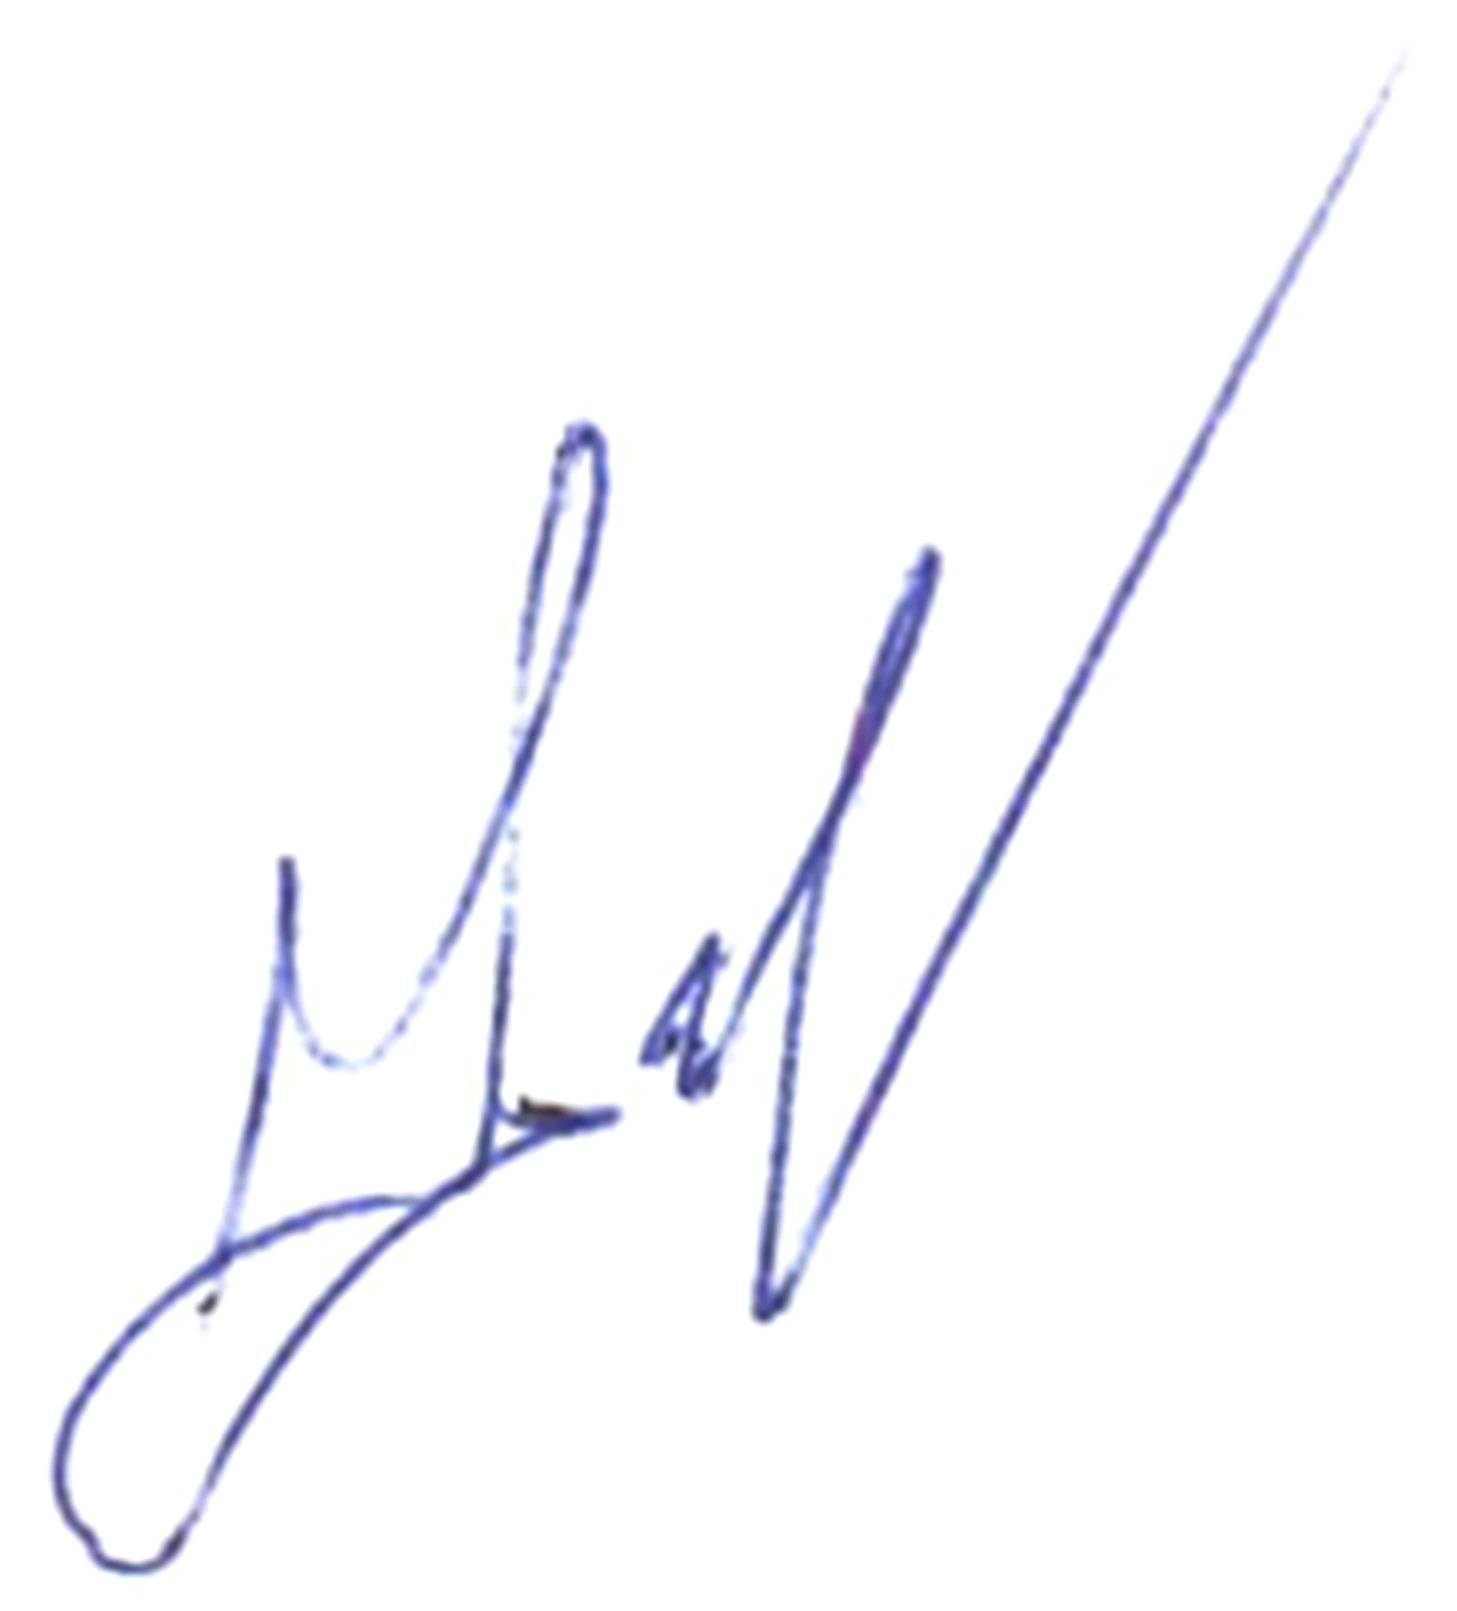
\includegraphics[width=2.3cm]{secretary-signature}
    &
    \defenseSecretaryFio
\end{tabularx} 
           % Титульный лист
\subsection*{Общая характеристика работы}

\newcommand{\actuality}{\underline{\textbf{Актуальность темы.}}}
\newcommand{\aim}{\underline{\textbf{Целью}}}
\newcommand{\tasks}{\underline{\textbf{задачи}}}
\newcommand{\defpositions}{\underline{\textbf{Основные положения, выносимые на~защиту:}}}
\newcommand{\novelty}{\underline{\textbf{Научная новизна:}}}
\newcommand{\influence}{\underline{\textbf{Практическая значимость}}}
\newcommand{\reliability}{\underline{\textbf{Достоверность}}}
\newcommand{\probation}{\underline{\textbf{Апробация работы.}}}
\newcommand{\contribution}{\underline{\textbf{Личный вклад.}}}
\newcommand{\publications}{\underline{\textbf{Публикации.}}}

{\actuality} 
% Актуальность - необходимо уметь контролировать рассеяние и поглощение,
% есть невидимость. Добавить 5 ссылок. Актуально сделать маскирующие
% покрытие на основе диэлектриков. 

В последние годы появилось большое количество работ по
нанофотонике~\cite{Tame-quantum-plasmonics-2013,
  Javier-graphene-plasmonics-2014, Khurgin-loss-plasmonics-2015,
  He-tunable-terahertz-graphene-metamaterials-2015,
  Segal-meta-nonlinar-PhC-2015,
  Poddubny-hyperbolic-metamaterials-2013, Kildishev-metasurface-2013}.
Высокая актуальность полученных результатов связана с перспективами их
практического применения и обусловлена стремительным развитием
нанотехнологий, что даёт возможность экспериментальной проверки
предлагаемых идей и подходов. Среди прочих, стоит отметить вопрос о
взаимодействии света с многослойной сферической наночастицей. Он
рассматривается в ряде прикладных задач, таких как: лечение
рака~\cite{Zhang-2010, Hirsch-2003}, различные методы диагностики в
медицине~\cite{Allain-2002}, разработка маскирующих суб-волновых
покрытий для видимого и микроволнового диапазонов~\cite{Qui-2009,
  Semouchkina-2013}, устройства плазмоники~\cite{Martin-2013,
  Alu-2005}, изучение тепловых свойств изоляторов~\cite{Xie-2013},
повышение эффективности солнечных элементов~\cite{Kameya-2011,
  Mann-2011} и так далее. Всё вместе это обуславливает актуальность
настоящей работы, в которой сперва излагается общий принцип,
позволяющий управлять рассеянием и поглощением электромагнитных волн
многослойными сферическими наночастицами, а потом идёт апробация на
частных примерах: минимизация рассеяния от идеально проводящей сферы
(частичная невидимость) и управление поглощением плазмонной частицы
$Si/Ag/Si$.

\underline{\textbf{Основные методы исследования.}}
Теория Ми~\cite{Mie-1908} входит в число основных инструментов применяемых
при анализе задач рассеяния и поглощения плоской электромагнитной
волны сферическими объектами. Эта теория была обобщённа на случай
многослойной сферы с произвольным числом слоёв~\cite{Yang-2003,
  Pena-scattnlay-2009} и доработана в настоящей работе, что позволило
реализовать её в виде комплекса программ для проведения компьютерного
моделирования. Достоинством теории является используемое ей разложение
поля по сферическим векторным гармоникам, что позволяет разделить
вклад в общее поле от электрического и магнитного дипольного
резонанса, а так же вклад резонансов квадруполя
и мультиполей более высокого порядка. Таким образом, становится
возможен анализ спектрального отклика многослойной сферы в зависимости
от её параметров (размеров и показателей преломления слоёв). Например,
в ряде случаев удаётся совместить в спектре рассеяния положение
нескольких резонансов (например, электрических дипольного и
квадрупольного), что создаёт эффект
суперрассеяния~\cite{Fan-2010,Fan-2011}. Аналогичный эффект
суперпоглощения подробно рассмотрен в настоящей работе.


 Как правило, при их решении возникает
необходимость оптимизации дизайна многослойной сферы (радиусов и
материальных параметров составных слоёв), обеспечивающего наилучшие
рабочие характеристики для каждого конкретного случая с учётом
фактических ограничений в предметной области.


\aim\ данной работы является разработка общего подхода к оптимизации
дизайнов многослойных сфер в рамках теории Ми, его последующая
реализация в комплексе компьютерных программ, выявление
закономерностей между дизайном многослойной сферы и её оптическими
свойствами.

Для~достижения поставленной цели необходимо было решить следующие {\tasks}:
\begin{enumerate}
  \item Разработать алгоритм для вычисления рассеяния и поглощения в
    многослойных сферических объектах и реализовать его в комплексе программ.
  \item Выбрать и реализовать алгоритм оптимизации, подходящий для
    работы с произвольными параметрами модели, описываемой обобщённой
    теорией Ми.
  \item Выявить основные закономерности взаимодействия с
    электромагнитной волной сферических маскирующих покрытий на
    основе диэлектриков.
  \item Исследовать эффект суперпоглощения света в многослойных
    сферических наночастицах.
\end{enumerate}



\defpositions
\begin{enumerate}
  \item Получены и реализованны в комплексе программ явные
    реккурентные соотношения для коэффициентов Ми в объёме
    многослойной сферы, выраженные через логарифмические производные
    функций Риккати-Бесселя увеличивающие численную стабильность.  
  
  \item Использование тонкого (размер мишени к размеру покрытия) диэлектриких многослойных покрытий позволяет
    уменьшить рассеяние от идеальное мишени в два раза.
  \item Использовать диэлектрикого порытия для небольшого объекта
    позволяет уменьшить рассеяние в 6 раз.

  \item TODO Использование алгоритма стохастической оптимизации методом
    адаптивной дифференциальной эволюции для решения задачи Ми
    позволяет выявлять семейства дизайнов с заранее заданными
    электромагнитными свойствами.

  \item Защищать цифры (уменьшили в два раза и т.д.). Показано, что
    маскирующие сферические покрытия из диэлектриков могут быть
    сконструированы, используя волноводоподобный эффект.  В этом
    случае при распространении внутри покрытия поле отстает по фазе от
    невозмущённой падающей волны на величину, кратную $2\pi$.
  \item Обнаружено семейство маскирующих сферических порытий из
    диэлектрических изотропных метаматериалов, реализующих эффект
    волнового обтекания.  Для получения заметного эффекта достаточно
    трёх слоёв в покрытии.
  \item В трёхслойных частицах $Si/Ag/Si$ возможно вырождение
    резонансных мультипольных откликов, приводящее к эффекту
    суперпоглощения, когда сечение поглощение оказывается больше, чем
    у bulk частицы. 
  \end{enumerate}

Положения соответствуют пункту 1 паспорта специальности 01.04.05 --
<<Оптика>> (Волновая (физическая) оптика. Интерференция, дифракция,
поляризация, когерентность света) по физико-математическим
наукам (представлены результаты фундаментальных исследований).

%\vspace{5.5em}
\novelty Используем диэлектрики для маскировки, использовать
оптимизация. Есть суперпоглощения.
\begin{enumerate}
  \item Впервые были получены явные реккурентные соотношения для
    коэффициентов Ми в многослойной сфере, выраженные через
    логарифмические производные функций Риккати-Бесселя. 
  \item Впервые метод дифференциальной эволюции был применён
    для изучения маскирующих сферических покрытий, показана высокая
    производительность метода.
  \item Было выполнено оригинальное исследование поглощения света
    наночастицами в режиме вырождения резонансых мультипольных откликов.
\end{enumerate}

\influence. Разработанные аналитические и численные методы для решения
уравнений Максвелла в рамках теории Ми, а так же реализующий их
программный комплекс с использованием стахостической оптимизации
методом дифференциальной эволюции могут быть использованы при
проектировании, оптимизации и анализе (включая анализ предельно
достижимых рабочих характеристик) широкого спектра устройств,
работающих как в оптическом, так и микроволновом диапазоне. Результаты
полученные при изучении поглощени света наночастицами могут быть
использованы при разработке инновационных устройств наноплазмоники,
фотоактивных катализаторов, красителей, поглощающих эмульсий и
аэрозолей.

Результаты диссертационной работы использовались при выполнении
грантов Министерства образования и науки РФ
(проект 11.G34.31.0020, гос. задание 2014/190, задание 3.561.2014/K),
Правительства РФ (грант 074-U01), РФФИ (грант 15-57-45141 ИНД\verb+_+а).


\reliability\ полученных результатов обеспечивается методическим
подходом на каждом этапе работы. Работа оптимизатора была проверена на
наборе стандартных тестовых функций. Аналитические результаты работы
были проверены в системе компьютерной алгебры (IPython). Компьютерная
реализация решения была проверена на наборе тестовых
задач. Аналитические результаты находятся в соответствии с
результатами, полученными другими авторами по теории Ми для случаев
однородной сферы и сферы с одним слоем покрытия.  Случаи большего
числа слоёв в покрытии сравнивался с коммерческими пакетами
моделирования, использующих численные методы конечных разностей во
временной области (Lumerical FDTD), метод конечных элементов (Comsol)
и метод конечных интегралов (CST MWS). Результаты по исследованию
маскирующих покрытий и поглощения света наночастицами находятся в
соответствии с результатами, полученными другими авторами для похожих
систем.

\probation\
Основные результаты работы докладывались~на:
перечисление основных конференций, симпозиумов и~т.\:п.

\contribution\ Автор принимал активное участие \ldots

%\publications\ Основные результаты по теме диссертации изложены в ХХ печатных изданиях~\cite{Sokolov,Gaidaenko,Lermontov,Management},
%Х из которых изданы в журналах, рекомендованных ВАК~\cite{Sokolov,Gaidaenko}, 
%ХХ --- в тезисах докладов~\cite{Lermontov,Management}.
 
\ifthenelse{\equal{\thebibliosel}{0}}{% Встроенная реализация с загрузкой файла через движок bibtex8
    \publications\ Основные результаты по теме диссертации изложены в XX печатных изданиях, 
    X из которых изданы в журналах, рекомендованных ВАК, 
    X "--- в тезисах докладов.%
}{% Реализация пакетом biblatex через движок biber
%Сделана отдельная секция, чтобы не отображались в списке цитированных материалов
    \begin{refsection}%
        \printbibliography[heading=countauthornotvak, env=countauthornotvak, keyword=biblioauthornotvak, section=1]%
        \printbibliography[heading=countauthorvak, env=countauthorvak, keyword=biblioauthorvak, section=1]%
        \printbibliography[heading=countauthorconf, env=countauthorconf, keyword=biblioauthorconf, section=1]%
        \printbibliography[heading=countauthor, env=countauthor, keyword=biblioauthor, section=1]%
        \publications\ Основные результаты по теме диссертации изложены в \arabic{citeauthor} печатных изданиях\nocite{bib1,bib2}, 
        \arabic{citeauthorvak} из которых изданы в журналах, рекомендованных ВАК\nocite{Ladutenko-cloak-2014,Ladutenko-Qabs-2015}, 
        \arabic{citeauthorconf} "--- в тезисах докладов\nocite{DD-14, MW-14}.%
    \end{refsection}
}
% При использовании пакета \verb!biblatex! для автоматического подсчёта
% количества публикаций автора по теме диссертации, необходимо
% их здесь перечислить с использованием команды \verb!\nocite!.
    

 % Характеристика работы по структуре во введении и в автореферате не отличается (ГОСТ Р 7.0.11, пункты 5.3.1 и 9.2.1), потому её загружаем из одного и того же внешнего файла, предварительно задав форму выделения некоторым параметрам

%Диссертационная работа была выполнена при поддержке грантов ...

%\underline{\textbf{Объем и структура работы.}} Диссертация состоит из~введения, четырех глав, заключения и~приложения. Полный объем диссертации \textbf{ХХХ}~страниц текста с~\textbf{ХХ}~рисунками и~5~таблицами. Список литературы содержит \textbf{ХХX}~наименование.

%\newpage
\subsection*{Содержание работы}
Во \underline{\textbf{введении}} обосновывается актуальность
исследований, проводимых в рамках данной диссертационной работы,
приводится обзор научной литературы по изучаемой проблеме,
формулируется цель, ставятся задачи работы, сформулированы научная
новизна и практическая значимость представляемой работы.

\underline{\textbf{Первая глава}} посвящена выбору универсального
алгоритма оптимизации и вопросам его практической
реализации. Сложность выбора обусловлена огромным количеством методов
оптимизации, а так же большим числом разновидностей каждого
метода. При выборе метода применительно к задаче Ми были использованны
следующие предпосылки:
\begin{itemize}
\item Несмотря на то, что решение Ми является аналитическим и
  выражается в виде разложения в ряд по сферическим векторным
  гармоникам, одновременное нахождение производных для зависимости от
  радиуса и материального параметра оказывается громоздким даже в
  случае однородной сферы, что тем более верно для случая
  произвольного числа сферических слоёв.  В связи с чем метод
  оптимизации не должен требовать для своей работы нахождения значений
  производных оптимизируемой функции.  Это особено актуально в случае,
  когда одновременно оптимизируются и толщина, и показатель
  преломления каждого слоя, или, например, оптимизируемая величина
  берётся в нескольких точках спектра одновременно.  Более того, могут
  возникать задачи, когда требуется оптимизировать значение поля внутри
  или рядом с конструируемой частицей.
\item Решение образовано быстро-осциллирующими функциями и, как
  следствие, будет содержать большое количество локальных
  экстремумов. Таким образом, алгоритмы оптимизации, требующие особого
  отношения к подобным случаям, оказываются заведомо менее
  производительными.
\item Параметры оптимизации (толщина и показатель
  преломления каждого слоя), а так же оптимизируемая величина
  (например эффективность рассеяния) являются
  вещественными числами.
\end{itemize}

Всё вместе это позволяет ограничить выбор стахостическими методами,
среди которых наиболее распространёнными являются генетические
алгоритмы, методы роя частиц и методы дифференциальной эволюции.  Эти
алгоритмы используют метод <<проб и ошибок>>.  Несколько пробных
решений (называемых индивидами) генерируются случайным образом и
многократно улучшаются с надеждой найти некое удовлетворительное
решение. Качество решения оценивается целевой функцией, возникшей из
задачи, которую предстоит оптимизировать.  Полная группа индивидов
называется популяцией.  Состояние популяции на конкретном шаге
итерации называется поколением.  Переход между поколениями
осуществляется в соответствии с рядом относительно простых правил,
которые составляют сущность определённого алгоритма.

Генетические алгоритмы обычно рассматривают вещественные числа в виде
набора битов.  В отличие от них, методы роя частиц и методы
дифференциальной эволюции могут работать в непрерывном пространстве
вещественных входных параметров естественным образом (используя
возможность сложения и вычитания векторов пробных решений), что делает
их гораздо более удобными для решения физических и инженерных
задач.  Производительность этих алгоритмов зависит от правильного
выбора значений некоторых внутренних параметров
алгоритма.  Использование адаптивных версий алгоритмов упрощает задачу
оптимизации: значения внутренних параметров настраиваются
автоматически при переходе между поколениями. Как правило, адаптивным
алгоритмам нужно гораздо меньше (более чем на порядок) итераций, чем
неадаптивным, чтобы добиться того же результата оптимизации.

В настоящей работе был использован алгоритм JADE+ с улучшенной
скоростью скрещивания (по алгоритму PMCRADE), который является
адаптивным вариантом алгоритма дифференциальной эволюции. Он имеет
явное преимущество перед адаптивной оптимизацией методом роя частиц в
ряде стандартных тестов.  Выполненная в рамках настоящей работы
реализация указанного метода позволяет эффективно использовать
современные процессоры с большим количеством параллельных потоков
вычисления и может выполняться на суперкомпьютерных кластерах с
использованием стандарта Message Parsing Interface (MPI).
Разработанное программное обеспечение успешно проходит набор
стандартных тестов для алгоритмов оптимизации.  Было получено
свидетельство о государственной регистрации программы для
ЭВМ~№2014611568.  Исходные тексты реализации алгоритма доступны для
скачивания на сайте \verb+https://github.com/kostyfisik/jade+

\underline{\textbf{Вторая глава}} посвящена доработке теории Ми для
случая многослойной сферы, последующей реализации полученной
математической модели в комплексе программ и верификации результатов
работы.

Более 100 лет назад Густав Ми опубликовал свою оригинальную работу о
взаимодействии плоской электромагнитной волны с однородной сферой.
Изложенная в ней теория впоследствии получила его имя и в настоящее
время входит в число основных инструментов применяемых при анализе
задач рассеяния и поглощения сферическими объектами.  Несмотря на
более чем вековую историю теории Ми, работы по её дальнейшему развитию
ведутся и в настоящее время.  Рядом авторов были предложены
математические модели, позволяющие изучать многослойные сферы с
произвольным числом слоёв.  Основная сложность при этом возникает при
численной реализации этих моделей.  В теории Ми решение для
рассеянного поля выражается в виде разложения в ряд:
\begin{align*}
{\rm \mathbf{E}}_s &=\sum_{n=1}^{\infty} E_n \left( i a_n {\rm
    \mathbf{N}}_{e1n}^{(3)} - b_n{\rm\mathbf{M}_{o1n}^{(3)}} \right),\\
\end{align*}
\begin{align*}
{\rm \mathbf{H}}_s &=\frac{k}{\omega\mu}
 \sum_{n=1}^{\infty} E_n \left( i b_n {\rm
    \mathbf{N}}_{o1n}^{(3)} + a_n{\rm\mathbf{M}_{e1n}^{(3)}} \right),  
\end{align*}
где $E_n=i^nE_0(2n+1)/n(n+1)$, $n$ порядок мультиполя, $E_0$ амплитуда
падающего поля, $a_n$ и $b_n$ коэффициенты разложения, соответствующие
электирческим и магнитным мультиполям, ${\rm \mathbf{N}}_{e1n}^{(3)}$,
${\rm \mathbf{N}}_{o1n}^{(3)}$, ${\rm\mathbf{M}_{o1n}^{(3)}}$ и
${\rm\mathbf{M}_{e1n}^{(3)}}$ это сферические векторные гармоники,
выражающиеся через тригонометрические функции, полимномы Лежандра и
сферические функции Бесселя и Ханкеля, $k$ и $\omega$ волновой вектор
и частота падающей волны, $\mu$ магнитная проницаемость в вакууме.
Поле внутри $l$-ого слоя стратифицированной сферы выражается
аналогичным образом TODO cite Yang:
\begin{align*}
{\rm \mathbf{E}}_l &=\sum_{n=1}^{\infty} E_n \left(
                     c_n^{(l)}{\rm\mathbf{M}}_{o1n}^{(1)}
                     -i d_n^{(l)} {\rm \mathbf{N}}_{e1n}^{(1)}
                     +i a_n^{(l)} {\rm \mathbf{N}}_{e1n}^{(3)}
                     - b_n^{(l)}{\rm\mathbf{M}}_{o1n}^{(3)} 
                     \right),\\
{\rm \mathbf{H}}_l &=\frac{k_l}{\omega\mu} \sum_{n=1}^{\infty} E_n
                     \left(
                      d_n^{(l)}{\rm\mathbf{M}}_{e1n}^{(1)} 
                     +i c_n^{(l)} {\rm \mathbf{N}}_{o1n}^{(1)} 
                     -i b_n^{(l)} {\rm \mathbf{N}}_{o1n}^{(3)} 
                     - a_n^{(l)}{\rm\mathbf{M}}_{e1n}^{(3)} 
                     \right),  
\end{align*}
где для каждого слоя определены коэффициенты разложения $d_n^{(l)}$ и
$c_n^{(l)}$ электрического и магнитного поля для входящего поля и,
аналогично, $a_n^{(l)}$ и $b_n^{(l)}$ для исходящего поля.  Связь
между всеми коэффициентами разложения можно выразить в виде системы
реккурентных уравнений, которые получаются из граничных условий между
слоями на напрерывность номальных компонент полей TODO cite Yang:
\begin{equation} % \tag{S} % tag - вписывает свой текст
  \label{eq:A2d1}
    % \begin{multlined}
    \begin{alignedat}{2}
d^{(l+1)}_{n}m_{l} \psi^{\prime}_{n}&{\left (m_{l+1} x_{l} \right )}
- a^{(l+1)}_{n} m_{l} \zeta^{\prime}_{n}{\left (m_{l+1} x_{l} \right )}\\
& - d^{(l)}_{n} m_{l+1} \psi^{\prime}_{n}{\left (m_{l} x_{l} \right )} 
+ a^{(l)}_{n} m_{l+1} \zeta^{\prime}_{n}{\left (m_{l} x_{l} \right )}
= 0,
\end{alignedat}
\end{equation}
\begin{equation} % \tag{S} % tag - вписывает свой текст
  \label{eq:A2d2}
\begin{alignedat}{2}
c^{(l+1)}_{n} m_{l} \psi_{n}&{\left (m_{l+1} x_{l} \right )}
  - b^{(l+1)}_{n} m_{l} \zeta_{n}{\left (m_{l+1} x_{l} \right )}\\
&- c^{(l)}_{n} m_{l+1} \psi_{n}{\left (m_{l} x_{l} \right )} 
+b^{(l)}_{n} m_{l+1} \zeta_{n}{\left (m_{l} x_{l} \right )}  =0,
\end{alignedat}
\end{equation}
\begin{equation} % \tag{S} % tag - вписывает свой текст
  \label{eq:A2d3}
\begin{alignedat}{2}
c^{(l+1)}_{n} \psi^{\prime}_{n}&{\left (m_{l+1} x_{l} \right )}
- b^{(l+1)}_{n} \zeta^{\prime}_{n}{\left (m_{l+1} x_{l} \right )}\\
&- c^{(l)}_{n} \psi^{\prime}_{n}{\left (m_{l} x_{l} \right )} 
+b^{(l)}_{n} \zeta^{\prime}_{n}{\left (m_{l} x_{l} \right )}   =0,
\end{alignedat}
\end{equation}
\begin{equation} % \tag{S} % tag - вписывает свой текст
  \label{eq:A2d4}
\begin{alignedat}{2}
 d^{(l+1)}_{n} \psi_{n}&{\left (m_{l+1} x_{l} \right )}
- a^{(l+1)}_{n} \zeta_{n}{\left (m_{l+1} x_{l} \right )}\\
& - d^{(l)}_{n} \psi_{n}{\left (m_{l} x_{l} \right )} 
+ a^{(l)}_{n} \zeta_{n}{\left (m_{l} x_{l} \right )}   =0,
\end{alignedat}
% \end{multlined}
\end{equation}
где $m_l$ показатель преломления в слое, нормированный на показатель
преломления окружающего пространства, $x_l$ параметр размера внешнего
радиуса слоя, $\psi_{n}(z) = z j_n(z)$ и $\zeta_{n}(z) = z h_n^1(z)$
функции Риккати-Бесселя, выраженные через сферические функции Бесселя
и Ханкеля.  Из выражений для падающей и рассеянной волны получаются
дополнительные условия на коэффициенты разложения
$c_n^{(L+1)}=d_n^{(L+1)}=1$, $a_n=a_n^{(L+1)}$ и $b_n=b_n^{(L+1)}$,
где $L$ общее число слоёв. Так как внутри центального слоя $l=1$ нет
рассеяния и, соответственно, исходящего поля, то
$a_n^{(1)}=b_n^{(1)}=0$. Последнее условие является избыточным для
решения системы уравнений~(TODO \labelcref{eq:A2d1} cref \labelcref{eq:A2d1,eq:A2d2,eq:A2d3,eq:A2d4}) и поэтому оно было использовано для дополнительной
проверки самосогласованности работы компьютерной программе.  После
проведения необходимых алгебраических преобразований значения
коэффициентов разложения были получены в явном виде:
\begin{equation*}
a^{(l)} = \frac
{
    {D^{(1)}_{n}}{\left (m_{l} x_{l} \right )}
    T_1\left (m_{l+1} x_{l} \right )
    +
    T_3\left (m_{l+1} x_{l} \right )
    m_{l}/m_{l+1}
}
{
   \zeta_{n}\left (m_{l} x_{l} \right )
   U\left (m_{l} x_{l} \right )
}
\end{equation*}
\begin{equation*}
b^{(l)} = \frac
{
    {D^{(1)}_{n}}{\left (m_{l} x_{l} \right )}
    T_2\left (m_{l+1} x_{l} \right )
    m_{l}/m_{l+1}
    +
    T_4\left (m_{l+1} x_{l} \right )
}
{
   \psi_{n}\left (m_{l} x_{l} \right )
   U\left (m_{l} x_{l} \right )
}
\end{equation*}

\begin{equation*}
  U(z) =    {D^{(1)}_{n}}(z) - {D^{(3)}_{n}}(z)
\end{equation*}
\begin{equation*}
  T_1(z) =   a^{(l+1)}_{n}  \zeta_{n}(z) 
           - d^{(l+1)}_{n}  \psi_{n}(z)
\end{equation*}

\begin{equation*}
  T_3(z) =  d^{(l+1)}_{n}  D^{(1)}_{n}(z)  \psi_{n}(z) 
          - a^{(l+1)}_{n}  D^{(3)}_{n}(z)  \zeta_{n} (z)
\end{equation*}


\underline{\textbf{Третья глава}} посвящена исследованию 

В \underline{\textbf{четвертой главе}} приведено описание 

В \underline{\textbf{заключении}} приведены основные результаты работы, которые заключаются в следующем:
%% Согласно ГОСТ Р 7.0.11-2011:
%% 5.3.3 В заключении диссертации излагают итоги выполненного исследования, рекомендации, перспективы дальнейшей разработки темы.
%% 9.2.3 В заключении автореферата диссертации излагают итоги данного исследования, рекомендации и перспективы дальнейшей разработки темы.
\begin{enumerate}
  \item Предложен метод изучения экстремальных оптических свойств
    многослойных сферических наночастиц с помощью теории Ми и
    стохастической оптимизации. Высокая вычислительная
    производительность этого подхода позволила выявить несколько новых
    физических эффектов, связанных с рассеянием и поглощением
    электромагнитной волны на многослойных сферических наночастицах.
  \item В задаче рассеяния плоской волны на многослойной сфере
    получены явные рекуррентные соотношения для коэффициентов Ми в
    расчёте локальных полей, выраженные через логарифмические
    производные функций Риккати-Бесселя.  Эти соотношения были
    добавлены в компьютерную программу, выполняющую вычисления в
    рамках задачи Ми.
  \item Рассеяние от объекта из идеального проводника можно
    существенно уменьшить с помощью многослойного покрытия толщиной
    $0.15\lambda$, используя только изотропные диэлектрические
    материалы: в 2 и в 6 раз для объектов диаметром $1.5\lambda$ и
    $\lambda/1.5$ соответственно. Обнаружен пороговый характер
    уменьшения рассеяния в зависимости от толщины покрытия.
  \item % (TODO берем балошени без слов min-max-min)
    Среди разнообразных оптимизированных дизайнов маскирующих покрытий из
    изотропных материалов с $\varepsilon$ меньше единицы, состоящих из
    множества слоёв равной толщины, выявлена закономерность,
    позволяющая разрабатывать эффективные трёхслойные сферические
    покрытия с разными толщинами слоёв. Дополнительной особенностью
    таких покрытий является значительное увеличение области спектра, в
    которой наблюдается эффект маскировки, при сравнении с покрытиями
    из диэлектриков. 
    %%%%%% Спектр --- засада
  \item В трёхслойных частицах $Si/Ag/Si$ возможно вырождение
    мультипольных резонансов, приводящее к эффекту суперпоглощения,
    когда сечение поглощения оказывается больше, чем у однородной
    частицы того же размера из произвольного изотропного
    материала. Максимальная эффективность поглощения в
    рассматриваемой системе была получена для небольших двухслойных
    частиц с преобладающей ролью электрического дипольного резонанса.
\end{enumerate}



%\newpage
\ifthenelse{\equal{\thebibliosel}{0}}{% Встроенная реализация с загрузкой файла через движок bibtex8
  \renewcommand{\refname}{\large Публикации автора по теме диссертации}
  \nocite{*}
}{% Реализация пакетом biblatex через движок biber
}

\insertbiblioauthor                          % Подключаем Bib-базы
\ifthenelse{\equal{\thebibliosel}{0}}{% Встроенная реализация с загрузкой файла через движок bibtex8
  \renewcommand{\refname}{\large Список литературы}
}{% Реализация пакетом biblatex через движок biber
}
\insertbiblioother
%\insertbibliofull
         % Содержание автореферата

\end{document}